% vim: set tw=78 tabstop=4 shiftwidth=4 aw ai:
\documentclass{beamer}

\usepackage[utf8]{inputenc}    % diacritice
\usepackage[english]{babel}
\usepackage{color}      % highlight
\usepackage{alltt}      % highlight
\usepackage{graphicx}
\graphicspath{{img/}}
\usepackage{tikz}
\usetikzlibrary{arrows.meta,positioning,calc}

% Code listings
\usepackage{listings}
\lstset{basicstyle=\ttfamily\small,columns=fullflexible,breaklines=true}

\usepackage{hyperref}      % folosiți \url{http://...}
% sau \href{http://...}{Nume Link}
\usepackage{verbatim}

\mode<presentation>
{%
  \usetheme{Madrid}
  \usecolortheme{dolphin}
}

% Light, modern-ish blue palette
\definecolor{PrismBlue}{RGB}{0,114,188}
\setbeamercolor{structure}{fg=PrismBlue}
\setbeamercolor{frametitle}{bg=PrismBlue!10,fg=PrismBlue!90!black}
\setbeamercolor{block title}{bg=PrismBlue!15,fg=PrismBlue!90!black}
\setbeamercolor{block body}{bg=PrismBlue!3,fg=black}
\setbeamercolor{author in head/foot}{bg=PrismBlue!90,fg=white}
\setbeamercolor{title in head/foot}{bg=PrismBlue!80,fg=white}
\setbeamercolor{upper separation line foot}{bg=PrismBlue!40}
\setbeamercolor{lower separation line foot}{bg=PrismBlue!40}

% Încărcăm simbolurilor Unicode românești în titlu și primele pagini
% (Removed \PreloadUnicodePage: not available with standard utf8 inputenc)

% Arătăm numărul frame-ului
\newcommand{\frameofframes}{/}
\newcommand{\setframeofframes}[1]{\renewcommand{\frameofframes}{#1}}

\setframeofframes{of}
\makeatletter
\setbeamertemplate{footline}
{%
  \begin{beamercolorbox}[colsep=1.5pt]{upper separation line foot}
  \end{beamercolorbox}
  \begin{beamercolorbox}[ht=2.5ex,dp=1.125ex,%
    leftskip=.3cm,rightskip=.3cm plus1fil]{title in head/foot}%
    \leavevmode{\usebeamerfont{institute in head/foot}\insertshortinstitute}%
    \hfill%
    {\usebeamerfont{title in head/foot}\insertshorttitle}%
    \hfill%
    {\usebeamerfont{frame number}\usebeamercolor[fg]{frame number}\insertframenumber~\frameofframes~\inserttotalframenumber}
  \end{beamercolorbox}%
  \begin{beamercolorbox}[colsep=1.5pt]{lower separation line foot}
  \end{beamercolorbox}
}
\makeatother

\setbeamertemplate{navigation symbols}{}%remove navigation symbols

% 3 logos (bottom-right) on slides after the title slide
\newcommand{\CornerLogos}{%
  \raisebox{-0.1cm}{
\includegraphics[height=0.55cm]{logo-oficial-enupb_2.jpg}}\hspace{0.15cm}%
  \raisebox{-0.1cm}{
\includegraphics[height=0.55cm]{images.jpg}}\hspace{0.15cm}%
  \raisebox{-0.1cm}{
\includegraphics[height=0.55cm]{images.png}}%
}
\logo{\CornerLogos}

\title[Tickling x86\_64]{Tickling x86\_64: Detecting Emulator Inaccuracies Through CPU Instruction Forensics \& Fuzzing}
\subtitle{}
\author[Lafosse Louis]{\textbf{Lafosse Louis}\\
\scriptsize\texttt{louis.lafosse@stud.acs.upb.ro}\\
\textbf{Scientific Advisor: Adrian Razvan DEACONESCU}}
\date{June 2026}

\begin{document}

% Slide-urile cu mai multe părți sunt marcate cu textul (cont.)
\setbeamertemplate{frametitle continuation}[from second]

\begingroup
\setbeamertemplate{logo}{}
\begin{frame}[plain]
  \vspace{0.2cm}
  \begin{columns}[T,onlytextwidth]

    \begin{column}{0.34\textwidth}
      \centering
      
\includegraphics[height=1.2cm]{logo-oficial-enupb_2.jpg}\\[-0.2em]
      \scriptsize University POLITEHNICA of Bucharest
    \end{column}
    \begin{column}{0.33\textwidth}
      \centering
      
\includegraphics[height=1.2cm]{images.jpg}\\[-0.2em]
      \scriptsize Faculty of Automatic Control and Computers
    \end{column}
    \begin{column}{0.33\textwidth}
      \centering
      
\includegraphics[height=1.2cm]{images.png}\\[-0.2em]
      \scriptsize Computer Science and Engineering Department
    \end{column}
  \end{columns}

  \vspace{0.6cm}
  \titlepage
\end{frame}
\endgroup

\section{Project}
\begin{frame}{General project description}
  \begin{itemize}
    \item Goal: check if x86-64 CPU emulators behave like \textbf{real native hardware}
    \item Why it matters: malware analysis, exploit testing, and binary research often trust emulator results
    \item Problem: emulators usually run normal programs, but can fail on rare CPU edge cases
    \item Impact: these differences create \textbf{false negatives} and enable \textbf{anti-emulation / fingerprinting}
  \end{itemize}
\end{frame}

\section{Background}
\begin{frame}{Background and concepts}
  \begin{itemize}
    \item Native hardware is used as the \textbf{ground truth}
    \item A probe is a very small program or shellcode snippet that checks one CPU behavior
    \item Examples of tested behavior:
      \begin{itemize}
        \item x87 FPU status bits after stack overflow or empty-stack access
        \item \texttt{LAHF}: exact CPU flag materialization
        \item \texttt{IDIV} / \texttt{MOVDQA}: correct fault delivery
        \item \texttt{SGDT}, \texttt{SIDT}, \texttt{SMSW}: machine-state fingerprints
      \end{itemize}
  \end{itemize}
\end{frame}

\begin{frame}{Example probe: \texttt{IDIV} overflow}
  \vspace{-0.15cm}
  \begin{columns}[T,onlytextwidth]
    \begin{column}{0.56\textwidth}
      \centering
      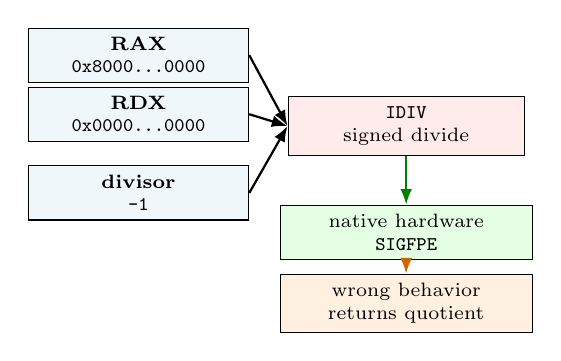
\begin{tikzpicture}[font=\scriptsize, every node/.style={align=center}]
        \node[draw,minimum width=2.8cm,minimum height=0.55cm,fill=PrismBlue!6]
          (rax) at (0,2.0) {\textbf{RAX}\\\texttt{0x8000...0000}};
        \node[draw,minimum width=2.8cm,minimum height=0.55cm,fill=PrismBlue!6]
          (rdx) at (0,1.25) {\textbf{RDX}\\\texttt{0x0000...0000}};
        \node[draw,minimum width=2.8cm,minimum height=0.55cm,fill=PrismBlue!6]
          (div) at (0,0.25) {\textbf{divisor}\\\texttt{-1}};

        \node[draw,minimum width=3.0cm,minimum height=0.75cm,fill=red!8]
          (idiv) at (3.4,1.1) {\textbf{\texttt{IDIV}}\\signed divide};

        \draw[-{Latex[length=2mm]},thick] (rax.east) -- (idiv.west);
        \draw[-{Latex[length=2mm]},thick] (rdx.east) -- (idiv.west);
        \draw[-{Latex[length=2mm]},thick] (div.east) -- (idiv.west);

        \node[draw,minimum width=3.2cm,minimum height=0.65cm,fill=green!10]
          (native) at (3.4,-0.25) {native hardware\\\textbf{\texttt{SIGFPE}}};
        \node[draw,minimum width=3.2cm,minimum height=0.65cm,fill=orange!12]
          (wrong) at (3.4,-1.15) {wrong behavior\\returns quotient};

        \draw[-{Latex[length=2mm]},thick,green!50!black] (idiv.south) -- (native.north);
        \draw[-{Latex[length=2mm]},thick,orange!80!black] (native.south) -- (wrong.north);
      \end{tikzpicture}

      \vspace{0.3em}
      \scriptsize
      Test idea: divide the smallest signed integer by \texttt{-1}. The mathematical
      result cannot be represented in 64 bits.
    \end{column}

    \begin{column}{0.44\textwidth}
      \begin{block}{What native hardware reports}
        \scriptsize
        \texttt{IDIV} overflow raises a divide-error exception, delivered by Linux as
        \textbf{\texttt{SIGFPE}}.

        \vspace{0.6em}
        Expected result: \textbf{\texttt{fault:8}}
      \end{block}

      \vspace{0.2em}
      \begin{itemize}
        \item QEMU and Blink matched native behavior in this probe
        \item Box64 returned a quotient instead of faulting
        \item This is a strong correctness bug because the native baseline is simple
      \end{itemize}
    \end{column}
  \end{columns}
\end{frame}

\section{Progress}
\begin{frame}{What changed in S2}
  \begin{itemize}
    \item Expanded the test suite from a few preliminary probes to a broader edge-case matrix
    \item Compared more instruction categories:
      \begin{itemize}
        \item x87, flags, timestamp counters, SSE alignment, MXCSR rounding, system-state instructions
      \end{itemize}
    \item Added clearer result labels:
      \begin{itemize}
        \item \textbf{Match}, \textbf{Mismatch}, \textbf{Unsupported}, \textbf{Internal bug}
      \end{itemize}
    \item Added \textbf{\texttt{sandsifter\_rs}} to search for new suspicious instruction sequences
  \end{itemize}
\end{frame}

\section{Overview}
\begin{frame}{Workflow: from fuzzing to stable tests}
  \vspace{-0.15cm}
  \begin{center}
    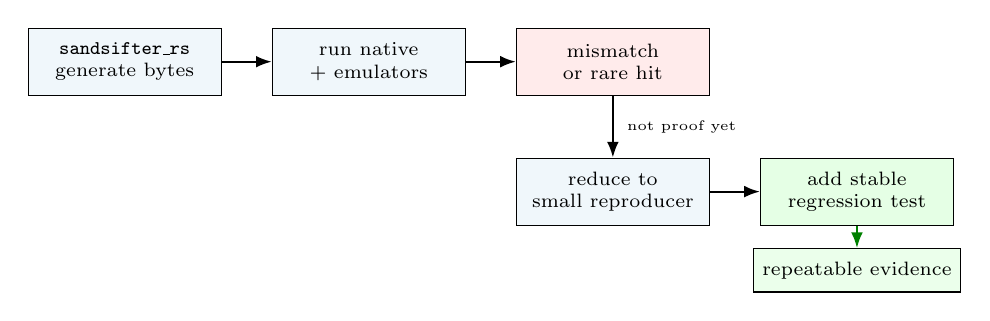
\begin{tikzpicture}[
      font=\scriptsize,
      box/.style={draw,minimum width=2.45cm,minimum height=0.85cm,fill=PrismBlue!6,align=center},
      warn/.style={draw,minimum width=2.45cm,minimum height=0.85cm,fill=red!8,align=center},
      good/.style={draw,minimum width=2.45cm,minimum height=0.85cm,fill=green!10,align=center},
      arrow/.style={-{Latex[length=2mm]},thick}
    ]
      \node[box] (fuzz) at (0,0) {\textbf{\texttt{sandsifter\_rs}}\\generate bytes};
      \node[box] (compare) at (3.1,0) {run native\\+ emulators};
      \node[warn] (lead) at (6.2,0) {mismatch\\or rare hit};
      \node[box] (reduce) at (6.2,-1.65) {reduce to\\small reproducer};
      \node[good] (test) at (9.3,-1.65) {add stable\\regression test};

      \draw[arrow] (fuzz) -- (compare);
      \draw[arrow] (compare) -- (lead);
      \draw[arrow] (lead) -- node[right,xshift=0.05cm] {\tiny not proof yet} (reduce);
      \draw[arrow] (reduce) -- (test);

      \node[draw,fill=green!8,minimum width=2.45cm,minimum height=0.55cm,align=center]
        (proof) at (9.3,-2.65) {repeatable evidence};
      \draw[arrow,green!50!black] (test) -- (proof);
    \end{tikzpicture}
  \end{center}

  \vspace{0.2cm}
  \begin{itemize}
    \item Fuzzing helps discover unknown edge cases
    \item The final report should rely on reduced, repeatable probes
  \end{itemize}
\end{frame}

\section{Results}
\begin{frame}{Result labels: how to read the matrix}
  \vspace{-0.1cm}
  \begin{center}
    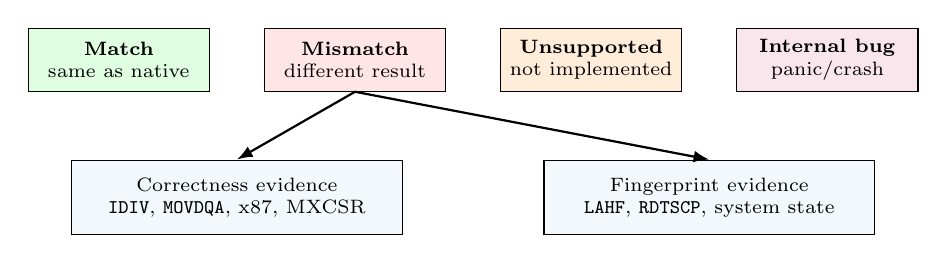
\begin{tikzpicture}[font=\scriptsize, every node/.style={align=center}]
      \node[draw,fill=green!12,minimum width=2.3cm,minimum height=0.8cm] (match) at (0,0) {\textbf{Match}\\same as native};
      \node[draw,fill=red!10,minimum width=2.3cm,minimum height=0.8cm] (mismatch) at (3,0) {\textbf{Mismatch}\\different result};
      \node[draw,fill=orange!15,minimum width=2.3cm,minimum height=0.8cm] (unsupported) at (6,0) {\textbf{Unsupported}\\not implemented};
      \node[draw,fill=purple!10,minimum width=2.3cm,minimum height=0.8cm] (bug) at (9,0) {\textbf{Internal bug}\\panic/crash};

      \node[draw,fill=PrismBlue!5,minimum width=4.2cm,minimum height=0.95cm] (correct) at (1.5,-1.75)
        {Correctness evidence\\\texttt{IDIV}, \texttt{MOVDQA}, x87, MXCSR};
      \node[draw,fill=PrismBlue!5,minimum width=4.2cm,minimum height=0.95cm] (finger) at (7.5,-1.75)
        {Fingerprint evidence\\\texttt{LAHF}, \texttt{RDTSCP}, system state};

      \draw[-{Latex[length=2mm]},thick] (mismatch.south) -- (correct.north);
      \draw[-{Latex[length=2mm]},thick] (mismatch.south) -- (finger.north);
    \end{tikzpicture}
  \end{center}

  \vspace{0.2cm}
  \begin{itemize}
    \item A mismatch is strongest when native behavior is exact and architecture-defined
    \item Some differences are deliberate synthetic state, but still useful for detection
  \end{itemize}
\end{frame}

\begin{frame}{Result summary by emulator family}
  \vspace{-0.1cm}
  \begin{columns}[T,onlytextwidth]
    \begin{column}{0.5\textwidth}
      \begin{block}{Linux user-mode}
        \scriptsize
        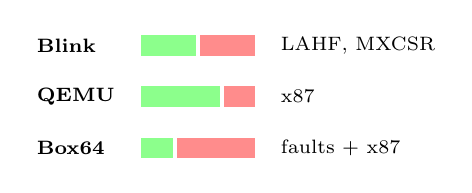
\begin{tikzpicture}[font=\scriptsize]
          \node[anchor=west] at (0,0) {\textbf{Blink}};
          \fill[green!45] (1.45,-0.13) rectangle (2.15,0.13);
          \fill[red!45] (2.2,-0.13) rectangle (2.9,0.13);
          \node[anchor=west] at (3.1,0) {LAHF, MXCSR};

          \node[anchor=west] at (0,-0.65) {\textbf{QEMU}};
          \fill[green!45] (1.45,-0.78) rectangle (2.45,-0.52);
          \fill[red!45] (2.5,-0.78) rectangle (2.9,-0.52);
          \node[anchor=west] at (3.1,-0.65) {x87};

          \node[anchor=west] at (0,-1.3) {\textbf{Box64}};
          \fill[green!45] (1.45,-1.43) rectangle (1.85,-1.17);
          \fill[red!45] (1.9,-1.43) rectangle (2.9,-1.17);
          \node[anchor=west] at (3.1,-1.3) {faults + x87};
        \end{tikzpicture}
      \end{block}
    \end{column}

    \begin{column}{0.5\textwidth}
      \begin{block}{Shellcode-only}
        \scriptsize
        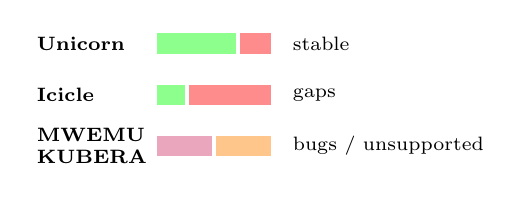
\begin{tikzpicture}[font=\scriptsize]
          \node[anchor=west] at (0,0) {\textbf{Unicorn}};
          \fill[green!45] (1.65,-0.13) rectangle (2.65,0.13);
          \fill[red!45] (2.7,-0.13) rectangle (3.1,0.13);
          \node[anchor=west] at (3.25,0) {stable};

          \node[anchor=west] at (0,-0.65) {\textbf{Icicle}};
          \fill[green!45] (1.65,-0.78) rectangle (2.0,-0.52);
          \fill[red!45] (2.05,-0.78) rectangle (3.1,-0.52);
          \node[anchor=west] at (3.25,-0.65) {gaps};

          \node[anchor=west,align=left] at (0,-1.3) {\textbf{MWEMU}\\\textbf{KUBERA}};
          \fill[purple!35] (1.65,-1.43) rectangle (2.35,-1.17);
          \fill[orange!45] (2.4,-1.43) rectangle (3.1,-1.17);
          \node[anchor=west] at (3.25,-1.3) {bugs / unsupported};
        \end{tikzpicture}
      \end{block}
    \end{column}
  \end{columns}

  \vspace{0.35cm}
  \begin{center}
    \scriptsize
    \textcolor{green!50!black}{green = matches} \quad
    \textcolor{red!70!black}{red = mismatches} \quad
    \textcolor{orange!80!black}{orange = unsupported} \quad
    \textcolor{purple!70!black}{purple = internal bugs}
  \end{center}
\end{frame}

\section{Plan}
\begin{frame}[plain]
  % subtle background accent
  
\begin{tikzpicture}[remember picture,overlay]
    \fill[PrismBlue!6] (current page.south west) rectangle ([yshift=2.2cm]current page.south east);
    \fill[PrismBlue!10] (current page.north west) rectangle ([yshift=-1.2cm]current page.north east);
  \end{tikzpicture}

  \vspace{0.1cm}
  \begin{center}
    \begin{minipage}{0.6\textwidth}
      \centering
      {\color{PrismBlue!90!black}\large\textbf{Next possible period}}
      \begin{itemize}
        \item Study the implementation on ARM64
        \item Add more emulator backends to \texttt{sandsifter\_rs}
        \item Check emulated env for:
          \begin{itemize}
            \item ESET, Kaspersky, Check Point
            \item Fortinet, Bitdefender
          \end{itemize}
      \end{itemize}
    \end{minipage}
  \end{center}

  \vfill
  \begin{center}
    \CornerLogos
  \end{center}
\end{frame}

\begin{frame}[plain]
  
\begin{tikzpicture}[remember picture,overlay]
    \fill[PrismBlue!6] (current page.south west) rectangle ([yshift=2.2cm]current page.south east);
    \fill[PrismBlue!10] (current page.north west) rectangle ([yshift=-1.2cm]current page.north east);
  \end{tikzpicture}

  \vfill
  \begin{center}
    {\color{PrismBlue!90!black}\fontsize{30}{34}\selectfont\textbf{Thank you}}\\[0.25em]
    {\Large\color{PrismBlue!80!black}Questions?}\\[0.8em]

    {\small\color{PrismBlue!70!black}
    \url{https://github.com/louislafosse/research-polytechnic}}
  \end{center}
  \vfill

  \begin{center}
    \CornerLogos
  \end{center}
\end{frame}

\end{document}
